\documentclass[a4paper]{scrartcl}
\usepackage[cm]{fullpage}
\usepackage{amsmath, amssymb, esint}
\usepackage{siunitx}

\usepackage{sectsty}
\sectionfont{\large\selectfont}
\subsectionfont{\normalsize\selectfont}

\usepackage{tikz, pgfplots}
\pgfplotsset{compat = 1.12}

\begin{document}

\title{PHYS3112: Zeeman Effect Prework}
\author{ \\ \\ }
\date{2017-05-16}
\maketitle

\section{Questions}
\subsection{What are the available magnetic sublevels \(m'\) of the lower level \(5s5p\) of Cd I?}
Since it only possesses an angular momentum quantum number of \(J = 1\), only \({-1, 0, 1}\) are available.

\subsection{Draw a graph showing the splitting of energy levels by an applied magnetic field \(B\) for the \(5s5d\) and \(5s5p\) levels of interest. Assume that \(g = 1\).}
\begin{center}
    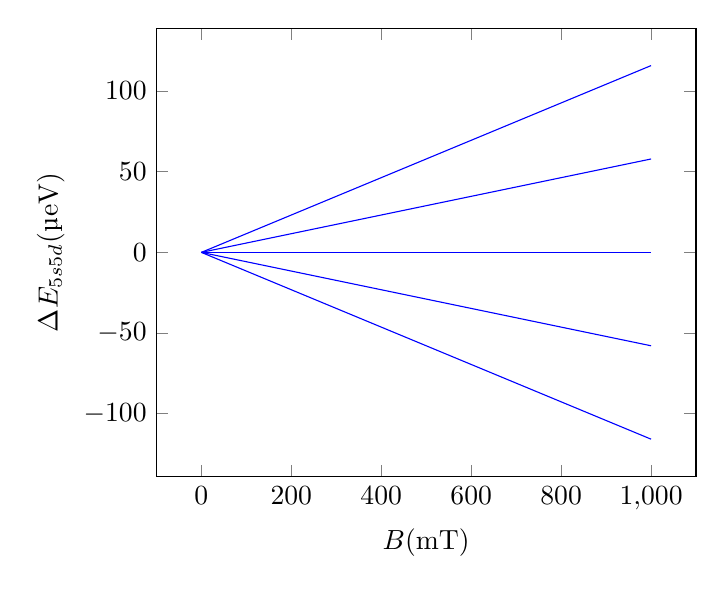
\begin{tikzpicture}
        \begin{axis}[
            xlabel = \(B (\si{\milli\tesla})\),
            ylabel = \(\Delta E_{5s5d} (\si{\micro\electronvolt})\)
        ]
            \addplot +[blue, no marks, smooth, domain = 0:1000] {5.788e-2 * x * -2};
            \addplot +[blue, no marks, smooth, domain = 0:1000] {5.788e-2 * x * -1};
            \addplot +[blue, no marks, smooth, domain = 0:1000] {5.788e-2 * x * 0};
            \addplot +[blue, no marks, smooth, domain = 0:1000] {5.788e-2 * x * 1};
            \addplot +[blue, no marks, smooth, domain = 0:1000] {5.788e-2 * x * 2};
        \end{axis}
    \end{tikzpicture}
    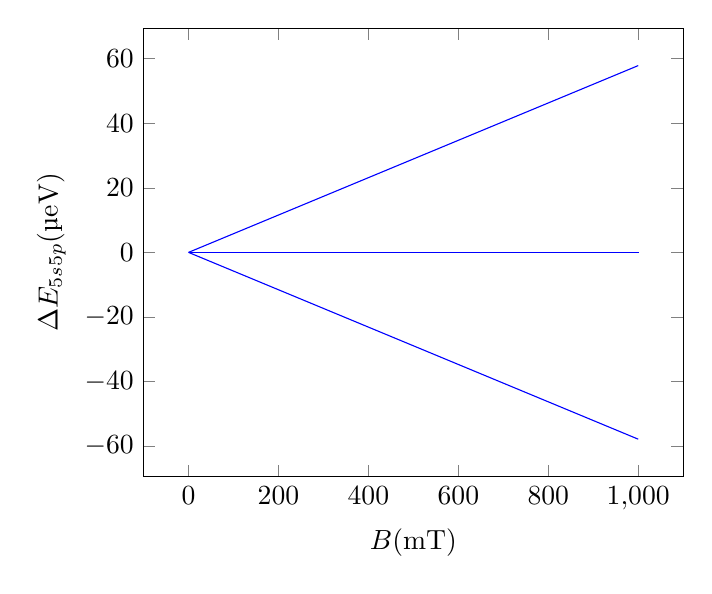
\begin{tikzpicture}
        \begin{axis}[
            xlabel = \(B (\si{\milli\tesla})\),
            ylabel = \(\Delta E_{5s5p} (\si{\micro\electronvolt})\)
        ]
            \addplot +[blue, no marks, smooth, domain = 0:1000] {5.788e-2 * x * -1};
            \addplot +[blue, no marks, smooth, domain = 0:1000] {5.788e-2 * x * 0};
            \addplot +[blue, no marks, smooth, domain = 0:1000] {5.788e-2 * x * 1};\
        \end{axis}
    \end{tikzpicture}
\end{center}

\subsection{Why are there only 3 red lines resulting from this transition?}
For an electric dipole transition (the most common type), only \(\Delta m = 0, \pm 1\) are allowed by the selection rules. Since the energy spacing between each energy level are constant, each of the allowed \(\Delta m\) correspond to one line.

\subsection{Calculate the energy shift and wavelength shifts in the transitions for a field of \SI{1}{\tesla}.}
The spacing between adjacent energy levels is \(\Delta E = \SI{57.88}{\micro\electronvolt}\).

The energy shifts for a transition for a \(\Delta m\) then becomes:
\[\Delta E_{\Delta m} = \Delta E \Delta m\]
which would be 0 and \(\pm\SI{57.88}{\micro\electronvolt}\) for the allowed transitions.

Wavelength shifts would then be:
\[\Delta \lambda = h c \left(\frac{1}{E + \Delta E} - \frac{1}{E}\right)\]
which would be 0 and \(\pm\SI{0.019}{\nano\metre}\) for the allowed transitions.

\subsection{Why would you only expect 2 lines when viewing parallel to the field direction?}
The \(\Delta m = 0\) transition acts as a dipole oscillating parallel to the field, so therefore does not radiate in the field direction, hence decreasing the number of lines observed.

\end{document}